\chapter{Bayesian Interpretations of English Tort Law}
\label{ch:tort}

\section{Epistemic responsibility}

The law of negligence asks what a reasonable person would have known and done. This is a question about beliefs and actions under uncertainty, and so, we argue, a question with a Bayesian answer. In our paper on Bayesian interpretations of English tort law we proposed that the core doctrines of negligence can be read as constraints on two things: on what a defendant ought to have believed, given the information available, and on what a defendant ought to have done, given those beliefs and the stakes \citep{polson_sokolov_tort}. We call the first epistemic responsibility and the second decision responsibility. Negligence is a failure of either.\index{epistemic responsibility}\index{negligence}

This chapter develops that reading across the elements of the tort. Duty of care asks whether the defendant was in a relationship that made harm to the claimant a foreseeable consequence of carelessness, a question about the probability of harm. Breach asks whether the defendant's conduct fell below the standard of the reasonable person, which we read as whether the defendant's choice failed to minimise expected cost, given beliefs that a reasonable person would have held. Causation asks whether the breach made a difference to the harm, a counterfactual probability. Remoteness asks whether the kind of harm was foreseeable, again a probability. Damages measure the loss. Each element maps onto a part of Bayesian decision theory.

\section{The reasonable person as a Bayesian agent}

In \emph{Blyth v Birmingham Waterworks} in 1856, Baron Alderson defined negligence as the omission to do something which a reasonable man, guided upon those considerations which ordinarily regulate the conduct of human affairs, would do, or doing something which a prudent and reasonable man would not do \citep{blyth1856}. The reasonable person has never been given a formal definition, and English judges have resisted attempts to supply one. But every case that discusses the standard asks the same questions: how likely was harm, how serious would it be, how costly was precaution, and what was the social value of the activity. These are the inputs to an expected cost calculation.\index{reasonable person}

\subsection{Probability: Bolton v Stone}

In \emph{Bolton v Stone}, decided by the House of Lords in 1951, a woman standing outside her house was struck by a cricket ball hit out of the ground \citep{bolton1951}. Balls had been hit out of the ground perhaps six times in thirty years, and none had previously injured anyone. The House held the club not liable. Lord Reid said that the test was whether the risk of damage to a person on the road was so small that a reasonable man in the position of the defendants, considering the matter from the point of view of safety, would have thought it right to refrain from taking steps to prevent the danger. The risk was foreseeable in the sense that it was not impossible; it was not material enough to require action.\index{Bolton v Stone}

The Bayesian reading is direct. The club's information was a history of about six balls leaving the ground in thirty seasons and no injuries. A reasonable estimate of the annual probability that a ball would strike a person on that road is the product of the rate of balls leaving the ground and the probability that a ball leaving the ground strikes a person. With a gamma prior on the rate and a beta prior on the strike probability (both defined, with their updating rules, in Appendix~\ref{app:toolkit}), the posterior expected annual probability of injury is small, perhaps a few in a thousand. The expected annual harm is that probability times the severity of an injury. The question for breach is whether a precaution, such as a higher fence, would have cost less than the expected harm it prevented over its life. Lord Reid's speech in \emph{Bolton} looks at the size of the risk alone and expressly declines to weigh the cost of precautions; the balance of risk against cost was read into the case by Lord Reid himself in \emph{The Wagon Mound (No 2)}, discussed below. The calculation above is our reading of the decision, not the reasoning of the House.

\subsection{Severity: Paris v Stepney}

In \emph{Paris v Stepney Borough Council} the claimant, who was already blind in one eye, lost the sight of his good eye when a chip of metal struck it at work \citep{paris1951}. The employer had not provided goggles. The House of Lords held the employer liable, because the consequences of an eye injury were far more serious for a one eyed worker than for others, even if the probability of injury was the same. Severity enters the expected harm multiplicatively; a precaution not justified for most workers may be justified for one whose loss would be total.

\subsection{Cost of precaution: Latimer v AEC}

In \emph{Latimer v AEC}, a factory floor flooded and became slippery; the employer spread sawdust but did not have enough to cover the whole floor; a worker slipped \citep{latimer1953}. The House of Lords held that the employer was not negligent in failing to close the factory, because the cost of doing so was out of proportion to the risk. The burden of precaution is the other side of the ledger.

\subsection{Social value: Watt v Hertfordshire}

In \emph{Watt v Hertfordshire County Council} a fireman was injured by a heavy jack that shifted in a lorry not designed to carry it, during an emergency response to a woman trapped under a vehicle \citep{watt1954}. Denning LJ said that one must balance the risk against the end to be achieved, and that saving life justifies taking considerable risk. The Compensation Act 2006 later permitted courts, in considering what steps a defendant should have taken, to have regard to whether a requirement to take them might prevent a desirable activity from being undertaken. The benefit of the activity enters the expected utility alongside its risk.

\subsection{The Hand formula}

These factors are combined in the formula Judge Learned Hand stated in \emph{United States v Carroll Towing} in 1947 \citep{carroll1947}: a defendant is negligent if $B < PL$, where $B$ is the burden of adequate precautions, $P$ the probability of the harm, and $L$ the gravity of the resulting injury. The formula is an expected cost comparison. Its marginal version, which Posner and others have emphasised, says that care should be increased until the marginal cost of care equals the marginal reduction in expected harm \citep{posner2014}. Let $x$ be the level of care, so that $B$ is now a function $B(x)$ giving its cost, and $P(x)$ the probability of harm. Optimal care minimises $B(x) + P(x)L$, and satisfies
\begin{equation}
B'(x^\ast) = -P'(x^\ast) L .
\label{eq:hand}
\end{equation}
Figure~\ref{fig:hand} illustrates. English courts do not cite the Hand formula as authority, and some judges have been critical of its apparent precision. But the factors they weigh are its factors, and the balance they strike is its balance.\index{Hand formula}\index{United States v Carroll Towing}

\begin{figure}[t]
\centering
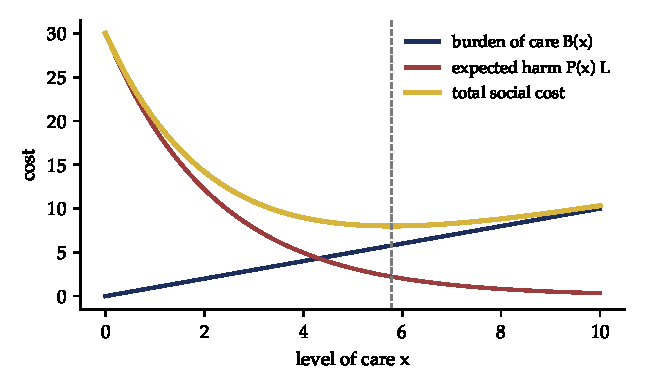
\includegraphics[width=\linewidth]{fig_hand}
\caption{The Hand formula in marginal form. The burden of care rises and the expected harm falls with the level of care. Total social cost is minimised where the slopes balance, marked by the dashed line.}
\label{fig:hand}
\end{figure}

\subsection{Where Bayes adds to Hand}

The Hand formula takes $P$ as given. Bayes asks where $P$ comes from. The reasonable person is not omniscient: the relevant probability is the one a reasonable person would have assessed using the information available, or reasonably obtainable, at the time. This has three consequences.

First, hindsight is excluded. After an accident, the probability that it would happen seems higher than it did before, because the accident has occurred. Courts warn against hindsight bias, and the Bayesian framework says precisely what is wrong with it: the accident is data that the defendant did not have, and the standard is the posterior given the defendant's information, not the information available after the accident.

Second, there is a duty to inquire. A defendant who could cheaply have obtained information that would have raised the assessed probability of harm is responsible for not obtaining it. This is a value of information calculation of the kind discussed in Chapter~\ref{ch:standards}. A manufacturer who fails to test a product, a landlord who fails to inspect wiring, an employer who ignores published research on an industrial disease, each has failed to buy information whose expected value exceeded its cost.

Third, the standard depends on the defendant's role. A professional is judged by the beliefs a reasonable member of the profession would hold. In \emph{Bolam v Friern Hospital Management Committee} the test was that a doctor is not negligent if he acted in accordance with a practice accepted as proper by a responsible body of medical opinion \citep{bolam1957}. In \emph{Bolitho} the House of Lords added that the body of opinion must be capable of withstanding logical analysis, in particular that the experts must have weighed the risks and benefits \citep{bolitho1998}. The Bayesian reading of \emph{Bolitho} is that professional practice is evidence about the reasonable posterior and the reasonable decision, but not conclusive evidence; a practice that does not reflect a coherent assessment of probabilities and utilities can be found wanting.

\section{Informed consent as expected utility}

In \emph{Montgomery v Lanarkshire Health Board} the Supreme Court held in 2015 that a doctor must take reasonable care to ensure that a patient is aware of any material risks involved in recommended treatment and of reasonable alternatives \citep{montgomery2015}. A risk is material if a reasonable person in the patient's position would be likely to attach significance to it, or if the doctor is or should be aware that this particular patient would. Nadine Montgomery, a diabetic woman of small stature, had not been told of the risk of shoulder dystocia in vaginal delivery, a risk of around nine to ten per cent for diabetic mothers, because her obstetrician judged that if told she would ask for a caesarean section.\index{Montgomery v Lanarkshire}

\emph{Montgomery} is an expected utility case. The patient, not the doctor, is the decision maker, and the patient's utilities govern. A risk is material if knowing it could change the patient's choice, which in decision terms means that the information has positive value of information for that patient. The doctor's duty is to supply information whose value to the patient exceeds the cost of supplying it, and the cost of a conversation is low. The obstetrician in \emph{Montgomery} effectively substituted her own utilities for the patient's, judging that a caesarean was worse than the patient would have judged it. The Supreme Court held that this was not her decision to make. Earlier, in \emph{Chester v Afshar}, the House of Lords had allowed recovery where a surgeon failed to warn of a small risk that then materialised, even though the patient might well have consented to the operation at a later date \citep{chester2004}. The case strains conventional causation, but it fits a view in which the patient's right to make an informed choice is itself protected.

\section{Causation}

\subsection{The but for test}

The claimant must prove that the breach caused the harm. The basic test is but for: would the harm have occurred if the defendant had not been negligent? In \emph{Barnett v Chelsea and Kensington Hospital Management Committee} a night watchman who had drunk tea laced with arsenic went to a casualty department and was sent home without examination \citep{barnett1969}. He died. The hospital was negligent, but the court found that he would probably have died even with proper treatment, because the antidote could not have been given in time. The claim failed on causation.\index{but for causation}

On the balance of probabilities the but for question becomes: is it more probable than not that the harm would not have occurred absent the breach? This is a counterfactual probability. Let $Y$ denote the harm, $Y(0)$ the harm that would have occurred without the breach and $Y(1)$ the harm with the breach. The claimant must show $\Prob(Y(0) = 0 \given Y(1) = 1, E) > 1/2$, where $E$ is the evidence. This probability is not identified by data in general, because we never observe both potential outcomes for the same person. It requires assumptions, and different assumptions give different answers. In the loss of a chance cases below, with $p_0$ the chance of a good outcome absent the breach, the all or nothing rule the courts applied is cruder than this: full recovery if $p_0 > 1/2$, nothing otherwise.

\subsection{Epidemiological evidence and the doubling of risk}

When causation must be inferred from population data, a common approach is the doubling of risk test. Suppose exposure to a substance multiplies the risk of a disease by $R$, the relative risk. Among exposed people who develop the disease, the fraction whose disease is attributable to the exposure is, under the assumption that exposure only adds cases and does not prevent or accelerate any,
\begin{equation}
\mathrm{PC} = 1 - \frac{1}{R}.
\label{eq:pc}
\end{equation}
This exceeds one half exactly when $R > 2$. Courts in England and the United States have used the test to decide whether epidemiology can establish causation on the balance of probabilities \citep{greenland1999}. Figure~\ref{fig:doubling} plots \eqref{eq:pc}.\index{doubling of risk}\index{probability of causation}

\begin{figure}[t]
\centering
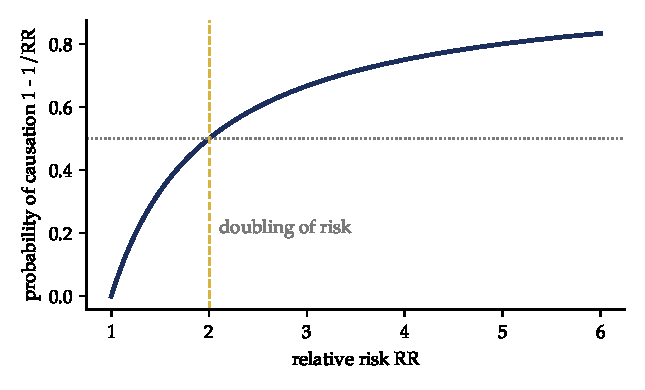
\includegraphics[width=\linewidth]{fig_doubling}
\caption{The probability of causation $1 - 1/R$ as a function of relative risk $R$. It crosses one half at $R = 2$, the doubling of risk.}
\label{fig:doubling}
\end{figure}

In \emph{Sienkiewicz v Greif} the Supreme Court considered the test in a mesothelioma case \citep{sienkiewicz2011}. Lord Phillips gave a careful account of the epidemiology, and several justices expressed doubt about deciding individual cases on statistical evidence alone. The court held that the doubling test is not a legal requirement for causation in mesothelioma cases. The Bayesian analysis explains the doubts. Equation \eqref{eq:pc} equals the probability of causation only under the assumption that exposure never prevents or accelerates disease, and is otherwise at best a lower bound (a lower bound if exposure can accelerate but never prevents disease); if exposure brings forward a disease that would have occurred later, the probability that the exposure was a cause, in the sense that the disease would not have occurred when it did, can be much larger. Greenland and Robins showed that the probability of causation is not identifiable from relative risks without further assumptions \citep{greenland1999}. The correct Bayesian response is to place a prior on the mechanism and report the posterior, recognising that the answer is assumption dependent. The court's discomfort can be read as a recognition of this dependence.

\subsection{Material contribution and Fairchild}

Mesothelioma is caused by asbestos fibres, but it is not known which fibre, or which exposure, triggers it, and a person exposed by several employers cannot prove which one caused the disease. In \emph{Fairchild v Glenhaven Funeral Services} the House of Lords held in 2002 that each employer whose negligence materially increased the risk was liable \citep{fairchild2002}. In \emph{Barker v Corus} it held that liability should be apportioned according to each employer's contribution to the risk \citep{barker2006}. Parliament promptly reversed \emph{Barker} for mesothelioma in section 3 of the Compensation Act 2006, restoring joint and several liability for the whole loss.\index{Fairchild v Glenhaven}\index{Barker v Corus}

The Bayesian analysis of \emph{Fairchild} is instructive. Suppose a worker was exposed by employers $A$, $B$, $C$ and $D$ in proportions $0.45, 0.30, 0.15, 0.10$ of total fibre dose, and suppose the risk of mesothelioma is proportional to cumulative dose. Then, given that the disease occurred, the posterior probability that it was caused by exposure from employer $j$ is proportional to that employer's dose (Figure~\ref{fig:fairchild}). No employer's probability exceeds one half, so none would be liable under the ordinary but for test, even though, if there is no background mesothelioma, it is certain that one of them caused the disease. The \emph{Fairchild} exception and the \emph{Barker} apportionment are two responses to this problem. \emph{Barker} is exactly the proportional, expected utility solution of Chapter~\ref{ch:standards}: each employer pays its expected share, and in aggregate the claimant is fully compensated if all are solvent. Section 3 of the 2006 Act chose instead to put the risk of insolvent defendants on the solvent ones.

\begin{figure}[t]
\centering
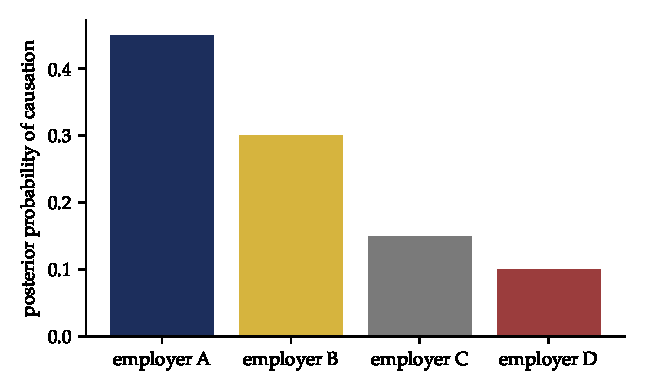
\includegraphics[width=\linewidth]{fig_fairchild}
\caption{Posterior probabilities of causation for four employers in a mesothelioma case, proportional to their shares of exposure. None exceeds one half, although their sum is one.}
\label{fig:fairchild}
\end{figure}

The earlier case of \emph{Wilsher v Essex Area Health Authority} illustrates the limits \citep{wilsher1988}. A premature baby developed retrolental fibroplasia; excess oxygen was one of five possible causes. The House of Lords refused to extend \emph{McGhee}, an earlier case about dermatitis that had allowed recovery on material increase in risk \citep{mcghee1973}, to a situation with several different possible agents. In Bayesian terms, \emph{Wilsher} involved competing causes with different mechanisms and unknown base rates, so the posterior probability that the oxygen was the cause could not be bounded away from small values. \emph{Fairchild} involved a single agent and several sources, so the probability that the agent was the cause was close to one, and only the allocation among sources was uncertain.

\section{Loss of a chance}

\subsection{Hotson and Gregg}

In \emph{Hotson v East Berkshire Area Health Authority} a boy fell from a tree and injured his hip; the hospital negligently failed to diagnose the injury for five days; he developed avascular necrosis \citep{hotson1987}. The trial judge found that even with prompt treatment there was a seventy five per cent chance he would have developed the condition, and awarded a quarter of the damages for the lost twenty five per cent chance. The House of Lords reversed: on the balance of probabilities the fall, not the delay, caused the necrosis, so the claim failed entirely.\index{loss of chance}\index{Hotson v East Berkshire}

In \emph{Gregg v Scott} a doctor negligently failed to refer a patient with a lump that turned out to be non Hodgkin lymphoma \citep{gregg2005}. The delay reduced his estimated chance of being cured, defined as surviving ten years disease free, from forty two per cent to twenty five per cent. A majority of the House of Lords held that he could not recover for the loss of a chance in a clinical negligence case. Since his chance of cure had never exceeded one half, it could not be shown that the negligence more probably than not caused the loss of a cure.\index{Gregg v Scott}

\subsection{The Bayesian analysis}

The majority in \emph{Gregg} treated the patient's outcome as determined, so that the question was whether he was one of the patients who would have been cured with prompt treatment. Lord Hoffmann put this sharply: the law regards the world as a deterministic place, and the question is what happened, not what the chances were. On that view, the forty two per cent was not a property of the patient but a statement of ignorance about which group he belonged to, and the claimant had to prove on the balance of probabilities that he was in the group who would have been cured and were not because of the delay.

The minority, Lord Nicholls and Lord Hope, held that the patient lost something of value, a chance of cure, and that he should be compensated for it. Lord Nicholls said that it would be irrational and indefensible for the law to recognise a forty five per cent chance as worth nothing when a fifty five per cent chance is worth the whole.

The Bayesian view is that the forty two per cent is the posterior probability of cure under prompt treatment, given everything known about the patient. Whether the world is deterministic is beside the point: the court must act on its probabilities, not on the unknown truth. The question is which remedy minimises expected loss across cases like this one. The all or nothing rule overcompensates claimants just above one half and undercompensates those below it. The proportional rule compensates each claimant by his expected loss and, aggregated across cases, compensates the class exactly. It also gives the right incentives to doctors: under the all or nothing rule a doctor whose negligence reduces patients' chances from forty to twenty per cent faces no liability at all, while one whose negligence reduces them from sixty to forty faces full liability. That is not a rational incentive structure. Our paper argues that the majority's reasoning in \emph{Gregg} rests on a mistaken view of what probability measures, and that proportional recovery is the coherent rule \citep{polson_sokolov_tort}.\index{proportional liability}

English law already accepts proportional recovery for lost chances in other settings. In \emph{Allied Maples v Simmons and Simmons} the claimant lost the chance of negotiating protection in a contract because of its solicitors' negligence \citep{alliedmaples1995}. The Court of Appeal held that where the outcome depended on the hypothetical action of a third party, the claimant need only show a substantial chance, and damages would be discounted by the probability. The distinction between clinical cases and cases depending on a third party's choice has never been convincingly explained. In French law, as Chapter~\ref{ch:commoncivil} discusses, \emph{perte de chance} is recognised in medical cases, and damages are proportional to the lost chance. The comparison is a good example of how two legal systems can reach different answers to a question that has a clear Bayesian solution.

\section{Remoteness and foreseeability}

In \emph{The Wagon Mound (No 1)} the Privy Council held that a defendant is liable only for damage of a kind that was reasonably foreseeable \citep{wagonmound1961}. Oil spilled from a ship in Sydney Harbour drifted to a wharf where welding was taking place, caught fire and damaged the wharf. The court found that fire was not a foreseeable consequence of the spill, because experts believed furnace oil on water could not be ignited. In \emph{The Wagon Mound (No 2)}, a different claimant on the same facts, with different evidence, the court found that a reasonable ship's engineer would have recognised a small but real risk of fire, and that since the risk could have been eliminated at no cost, the defendant was liable \citep{wagonmound1967}.\index{Wagon Mound}

The two cases differ in the evidence about the probability of fire and show that foreseeability is a probability judgment made on the evidence before the court. \emph{Wagon Mound (No 2)} also shows the Hand formula at work: a small probability suffices for liability when the precaution is costless. Lord Reid, reinterpreting \emph{Bolton v Stone}, distinguished it from the oil spill: there the risk was small and the precaution costly, here the risk was small and the precaution free. This balance of risk against cost is his gloss in \emph{Wagon Mound (No 2)}; the speech in \emph{Bolton} itself did not weigh cost.

\section{Duty of care}

The duty of care is the most normative element of negligence, and the one least amenable to a probabilistic reading. In \emph{Donoghue v Stevenson} Lord Atkin's neighbour principle said that one must take reasonable care to avoid acts or omissions which one can reasonably foresee would be likely to injure one's neighbour \citep{donoghue1932}. Foreseeability is again probability. In \emph{Caparo Industries v Dickman} the House of Lords added the requirements of proximity and that it be fair, just and reasonable to impose a duty \citep{caparo1990}. In \emph{Robinson v Chief Constable of West Yorkshire} the Supreme Court emphasised incremental development by analogy with established categories \citep{robinson2018}.\index{duty of care}\index{Caparo v Dickman}

Proximity and fairness are policy judgments, but they can be framed as judgments about incentives and about the allocation of losses, which brings them within decision theory. A duty that would expose auditors to indeterminate liability to anyone who reads their reports, the concern in \emph{Caparo}, would raise the cost of audits and might reduce their supply without improving their quality. The question is whether imposing the duty improves expected social welfare, a question that requires evidence about behaviour, not a fixed formula. Chapter~\ref{ch:misrep} develops this for the case of statements and advice.

\section{Contributory negligence and apportionment}

Under the Law Reform (Contributory Negligence) Act 1945, where a claimant suffers damage partly through his own fault, damages are reduced to the extent the court thinks just and equitable having regard to the claimant's share in the responsibility. Courts in practice apportion by a combination of causal potency and blameworthiness. A decision theoretic analysis suggests that apportionment should be chosen to give both parties efficient incentives, by reference to the incentives each party faces. In the standard bilateral care model of Shavell, however, negligence with a defence of contributory negligence, or comparative negligence, with due care standards set efficiently induces efficient care whatever the division of the loss \citep{shavell1987}. Apportionment therefore matters for incentives chiefly when the courts are uncertain about the standard, make errors, or when activity levels matter.

\section{Strict liability}

Some torts do not require negligence. Under \emph{Rylands v Fletcher}, a person who brings onto his land something likely to do mischief if it escapes is answerable for the damage it causes \citep{rylands1868}. Strict liability shifts the whole expected cost of an activity to the actor, who then chooses both the level of care and the level of activity efficiently (in the unilateral case; in the bilateral model, strict liability without a contributory negligence defence leaves the victim no incentive to take care). Negligence liability induces efficient care but not efficient activity levels, because the actor who takes due care escapes liability for the residual risk. Shavell's analysis of this distinction is a classic of law and economics \citep{shavell1987}. The Bayesian contribution is again about information: strict liability is attractive when the actor knows more than the court about the probability of harm, because it puts the decision in the hands of the party with the better posterior.

\section{Summary}

Negligence is a failure of epistemic or decision responsibility. Breach is a failure to minimise expected cost given reasonable beliefs; foreseeability and remoteness are probability judgments; causation is a counterfactual probability that requires modelling assumptions; and loss of a chance is a case where the all or nothing rule conflicts with the logic of expected loss. English tort law is more Bayesian than its judges usually admit, and where it departs from Bayesian reasoning, as in \emph{Gregg v Scott}, the departure is costly. Chapter~\ref{ch:misrep} applies the same framework to misrepresentation, where the defendant's beliefs, and what he said about them, are the subject of the claim.

\section*{Notes and Questions}
\addcontentsline{toc}{section}{Notes and Questions}
\begin{enumerate}[label=\arabic*.]
\item In \emph{Bolton v Stone}, suppose six balls left the ground in thirty seasons and that a ball leaving the ground strikes a person with probability $0.02$. With a gamma prior of shape one and rate one on the annual rate (Appendix~\ref{app:toolkit}), compute the posterior expected annual probability of injury. If an injury costs one hundred thousand pounds and a fence would cost fifty thousand pounds and last twenty years, was the club negligent on the Hand formula?
\item Show that if exposure can accelerate disease onset, the probability of causation can exceed $1 - 1/R$. Construct an example.
\item In the \emph{Fairchild} example, suppose employer $A$ is insolvent. Compare the claimant's recovery under \emph{Barker} apportionment and under section 3 of the Compensation Act 2006.
\item Under all or nothing and proportional rules, compute the expected liability of a doctor whose negligence reduces patients' chances of cure from $p_0$ to $p_1$, as functions of $p_0$ and $p_1$. Which rule gives incentives proportional to the harm done?
\item Write a short judgment in \emph{Gregg v Scott} adopting the Bayesian analysis. Address Lord Hoffmann's argument that the world is deterministic.
\item Explain why \emph{Montgomery} can be described as a value of information test.
\end{enumerate}

\section*{Further reading}
Our paper sets out the program of this chapter in more detail \citep{polson_sokolov_tort}. Shavell's \emph{Economic Analysis of Accident Law} remains the best economic treatment \citep{shavell1987}. On probability of causation, Greenland and Robins \citep{greenland1999}. Lord Phillips's speech in \emph{Sienkiewicz} is a rare judicial engagement with epidemiology \citep{sienkiewicz2011}.
